\documentclass[aspectratio=1610]{beamer}

\usetheme{unnslides}
\usefonttheme{professionalfonts}

\usepackage{listings}
\usepackage{graphicx}
\usepackage{caption}
\usepackage{cmbright}
\usepackage{fontspec}
\usepackage{unicode-math}
\usepackage{amsfonts}
\usepackage{subfig}

\setromanfont{CMU Serif}
%\setsansfont{CMU Sans Serif}
\setmathfont{Latin Modern Math}

\usepackage{polyglossia}
%\setbeamertemplate{itemize item}{\color{black}$\blacktriangleright$}

\DeclareMathOperator*{\argmax}{arg\,max}
\DeclareMathOperator*{\argmin}{arg\,min}
\DeclareMathOperator{\sign}{sign}
\DeclareMathOperator{\re}{Re}

\graphicspath{ {../paper/images/}{img/} }
%set pages numeration
\setbeamertemplate{footline}[frame number]
\setbeamertemplate{headline}{}
\setlength\abovecaptionskip{-1pt}

\title{Parallel Multi-objective Optimization Method for Finding Complete Set of Weakly Efficient Solutions}
\author{\textbf{Vladislav~Sovrasov}}
\institute{Lobachevsky University of Nizhni Novgorod}
\date{}

\begin{document}
\begin{frame}[noframenumbering,plain]
\titlepage
\end{frame}

\begin{frame}
  \begin{center}
  \frametitle{Problem statement}

  \begin{displaymath}
    \min\{f(y): y\in D\}, D=\{y\in \mathbb{R}^n: a_i \leqslant y_i \leqslant b_i, 1\leqslant i \leqslant n \},
  \end{displaymath}
where \(f(y)\) is a vector-function.

\enspace
Solution of the problem is a set of non-dominated points (Slater set):
  \begin{displaymath}
    S(D) = \{y\in D: \nexists z\in D, f_i(z)<f_i(y),1\leqslant i \leqslant m\}
  \end{displaymath}
Assume objectives to satisfy Lipschitz condition in \(D\):
  \begin{displaymath}
    |f_i(y_1)-f_i(y_2)|\leqslant L_i\Vert y_1-y_2\Vert,y_1,y_2\in D,0<L_i<\infty,1\leqslant i\leqslant m
  \end{displaymath}

\end{center}
\end{frame}

\begin{frame}
  \frametitle{Dimension reduction}
  Peano-type curve \(y(x)\) allows to reduce dimension of the original multi-objective problem:
  \begin{gather}
    \lbrace y\in \mathbb{R}^N:-2^{-1}\leqslant y_i\leqslant 2^{-1},1\leqslant i\leqslant N\rbrace=\{y(x):0\leqslant x\leqslant 1\} \nonumber \\
    \min\{f(y): y\in D\}=\min\{f(y(x)): x\in [0,1]\} \nonumber
  \end{gather}

  \begin{figure}[ht]
    \subfloat{{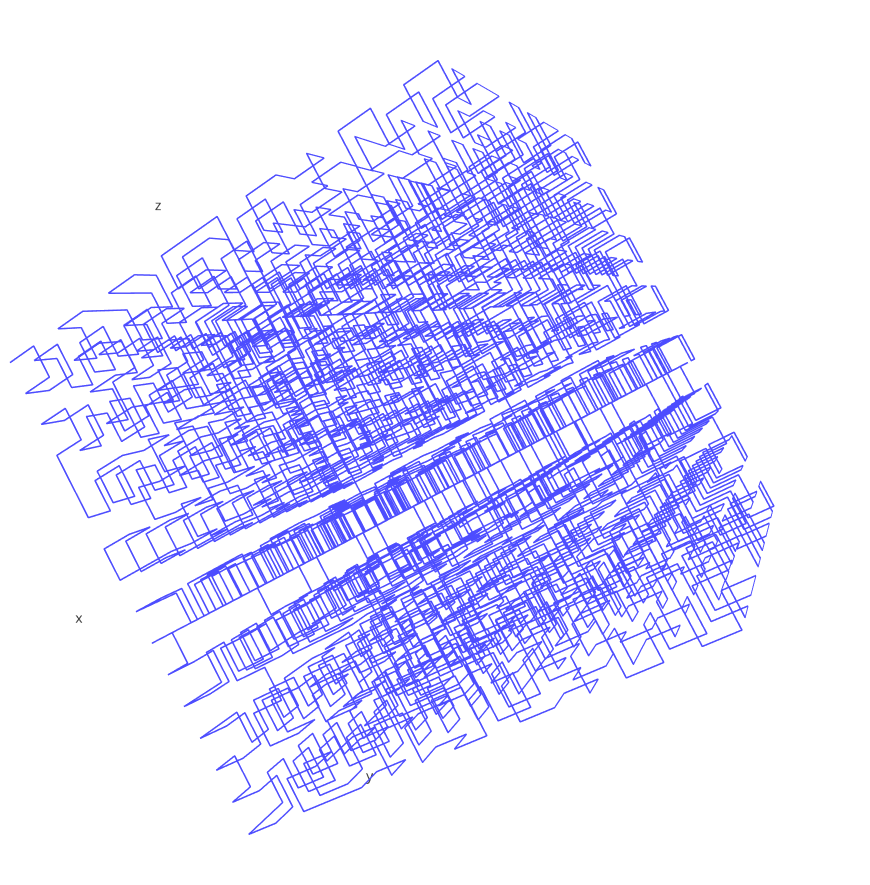
\includegraphics[width=.35\textwidth]{img/peano3d.png} }}
    \subfloat{{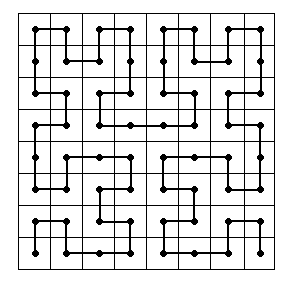
\includegraphics[width=.35\textwidth]{img/peano2d.png} }}
  \end{figure}
\end{frame}

\begin{frame}
  \frametitle{Scalarization tecnique}
  Multi-objective problem can be reduced to a scalar optimization problem using the following function:
  \begin{eqnarray*}
    h(x,y)=\min\{f_i(x)-f_i(y):1\leqslant i\leqslant m\}, \\
    \varphi(x)=\max\{h(x,y):y\in [0,1]\},x\in [0,1].
  \end{eqnarray*}
If \(x^*\) is weakly effective point, then \(\varphi(x^*)= 0\), in the opposite case \(\varphi(x^*)> 0\), so
the equivalent scalar problem is:
  \begin{displaymath}
    \varphi^*=\min\{\varphi(x):x\in [0,1]\}.
  \end{displaymath}
\end{frame}

\begin{frame}
  \frametitle{Scalarization tecnique}
  Example:
  \begin{figure}
    \subfloat{{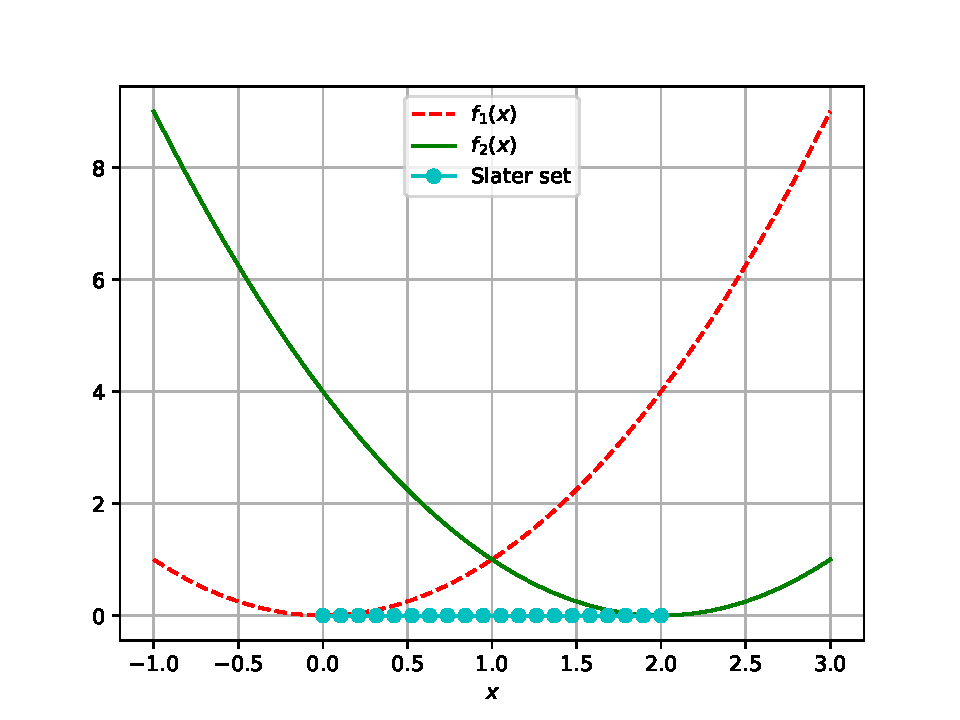
\includegraphics[width=.5\textwidth]{img/objectives.pdf} }}
    \subfloat{{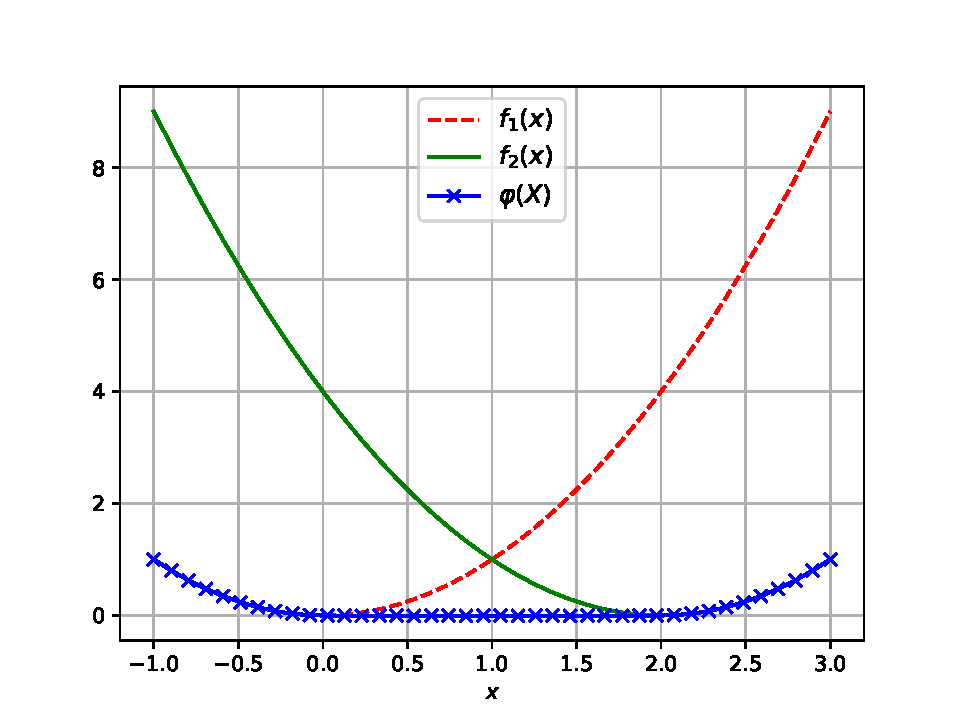
\includegraphics[width=.5\textwidth]{img/phi_func.pdf} }}
  \end{figure}
\end{frame}

\begin{frame}
  \frametitle{Optimization method}
Optimization method generates searh sequence \(\{x_k\}\) and consists of the following steps:
\begin{enumerate}
  \setlength{\itemindent}{.1in}
  \item[Step 1.] Sort the searh information (one-dimentional points) in increasing order.
  \item[Step 2.] Compute an approximation of the function \(\varphi(x)\).
  \item[Step 3.] For each interval \((x_{i-1}, x_i)\) compute quantity \(R(i)\), called characteristic.
  \item[Step 4.] Choose an interval \((x_{t-1}, x_t)\) with the greatest characteristic and
  compute objective \(f(y(x))\) in the point choosen using the descision rule \(d\):
  \begin{displaymath}
    x^{k+1}=d(t)\in (x_{t-1}, x_t)
  \end{displaymath}
  \item[Step 5.] If \(x_{t}-x_{t-1}<\varepsilon\) stop the method.
\end{enumerate}
\textit{\footnotesize	{Detailed description: Strongin R.G., Sergeyev Ya.D.: Global optimization with non-convex constraints. Sequential and parallel algorithms (2000), Chapter 7}}
\end{frame}

\begin{frame}
  \frametitle{Improved parallel optimization method}
  \begin{itemize}
    \item
    \textit{Local refinement.} Every \(q\) iterations ignore the characteristics \(R(i)\)
    and perform calculation of the objective near the current running-minimum point of the \(\varphi(x)\) approximation.
    \item
    \textit{Parallelization by characteristics.} At the Step 4 choose \(p\) best intervals
    and generate \(p\) new points using rule \(d(i)\). Then compute the objective \(f(y(x))\) at these
    points in parallel exploiting \(p\) computation units.

    \enspace
    In the best case (method doesn't generate redundand points compared to sequental
    one and wastes time only on computation of the objective)
    this scheme can give speedup in \(p\) times.
  \end{itemize}

\end{frame}

\begin{frame}
  \frametitle{Results}
  The method was implemented on C++ language using OpenMP framework. All the experimants were carried out on
  2xIntel Sandy Bridge E5-2660 2.2 GHz (total 16 cores) with 64Gb RAM.

  Examples of numerical solutions:
  \begin{figure}[ht]
      \centering
      \subfloat{{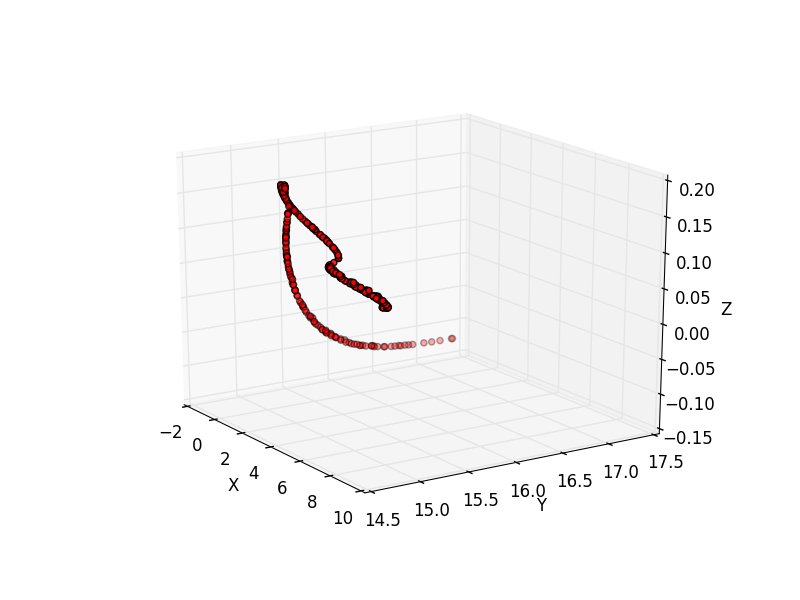
\includegraphics[width=.5\textwidth]{../img/viennet.png}}}
      \subfloat{{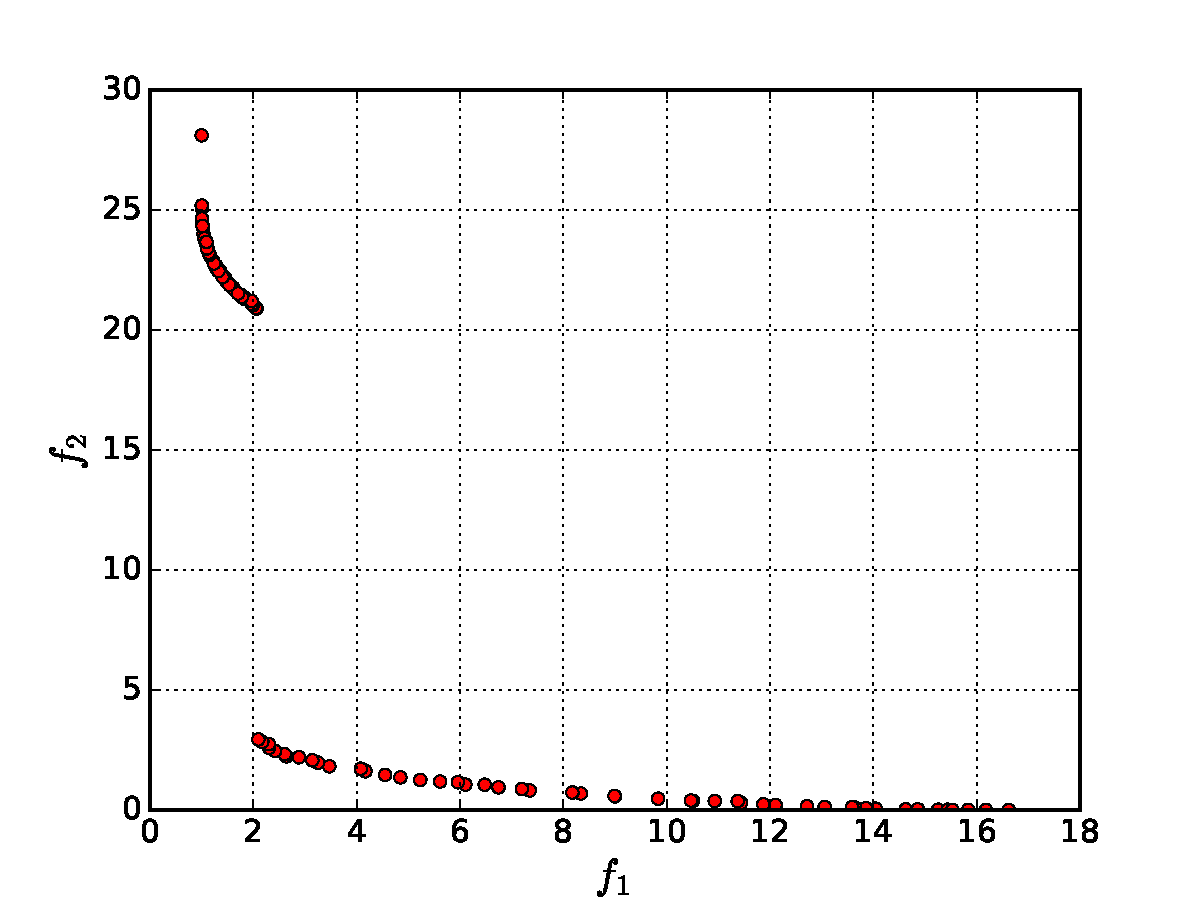
\includegraphics[width=.5\textwidth]{../img/poloni.pdf} }}
  \end{figure}
\end{frame}

\begin{frame}
  \frametitle{Results}

  Number of iterations decreases when increasing number of threads \(p\).
  \begin{table}
    \centering
    \begin{tabular}{|l|p{1.5cm}|p{1.5cm}|p{1.5cm}|p{1.5cm}|p{1.5cm}|}
  \hline
  \textbf{Problem} & \multicolumn{5}{c|}{\(p\)}\\
  \cline{2-6}
    & \(1\) & \(2\) & \(4\) & \(8\) & \(16\)\\
  \hline
  Markin-Strongin & 1041(198) & 516(198) & 256(185) & 131(197) & 68(191) \\
  \hline
  Fonseca and Fleming 2d & 1181(93) & 636(99) & 386(111) & 176(95) & 106(97) \\
  \hline
  Fonseca and Fleming 3d & 5346(160) & 3551(183) & 1186(143) & 606(153) & 351(142) \\
  \hline
  Viennet problem & 4896(276) & 2156(273) & 1226(270) & 631(287) & 286(274)\\
  \hline
  Poloni's function & 3351(102) & 1706(90) & 856(88) & 426(96) & 201(99) \\
  \hline
  \end{tabular}
  \end{table}

\end{frame}

%\begin{frame}
%  \frametitle{Results (speedup in iterations)}
%  \begin{table}
%    \centering
%    \begin{tabular}{|l|p{1.5cm}|p{1.5cm}|p{1.5cm}|p{1.5cm}|}
%  \hline
%  \textbf{Problem} & \multicolumn{4}{c|}{\(p\)}\\
%  \cline{2-5}
%    & \(2\) & \(4\) & \(8\) & \(16\)\\
%  \hline
%  Markin-Strongin & 2.02 & 4.07 & 7.95 & 15.31 \\
%  \hline
%  Fonseca and Fleming 2d & 1.86 & 3.06 & 6.71 & 11.14 \\
%  \hline
%  Fonseca and Fleming 3d & 1.51 & 4.51 & 8.82 & 15.23 \\
%  \hline
%  Viennet problem & 2.27 & 3.99 & 7.76 & 17.12\\
%  \hline
%  Poloni's problem & 1.96 & 3.91 & 7.87 & 16.67 \\
%  \hline
%  \end{tabular}
%  \end{table}
%
%\end{frame}
%
\begin{frame}
  \frametitle{Results (speedup in time)}
  Each calculation of the objective takes about 8ms.
  \begin{table}[ht]
    \centering
    \begin{tabular}{|l|p{1.6cm}|p{1.5cm}|p{1.5cm}|p{1.5cm}|p{1.5cm}|}
  \hline
  \textbf{Problem} & \multicolumn{5}{c|}{\(p\)}\\
  \cline{2-6}
  &\(1\)(time, s) & \(2\) & \(4\) & \(8\) & \(16\)\\
  \hline
  Markin-Strongin & 104.47 & 1.97 & 3.65 & 6.79 & 9.90 \\
  \hline
  Fonseca and Fleming 2d & 118.95 & 1.85 & 2.81 & 5.79 & 6.40 \\
  \hline
  Fonseca and Fleming 3d & 554.45 & 1.51 & 4.14 & 8.05 & 10.69 \\
  \hline
  Viennet problem & 1488.6 & 2.22 & 3.64 & 6.98 & 13.49\\
  \hline
  Poloni's problem & 336.74 & 1.82 & 3.64 & 6.98 & 10.60 \\
  \hline
  \end{tabular}
  \end{table}
\end{frame}

\begin{frame}
  \frametitle{Results (speedup and efficiency)}
  \begin{figure}[ht]
      \centering
      \subfloat{{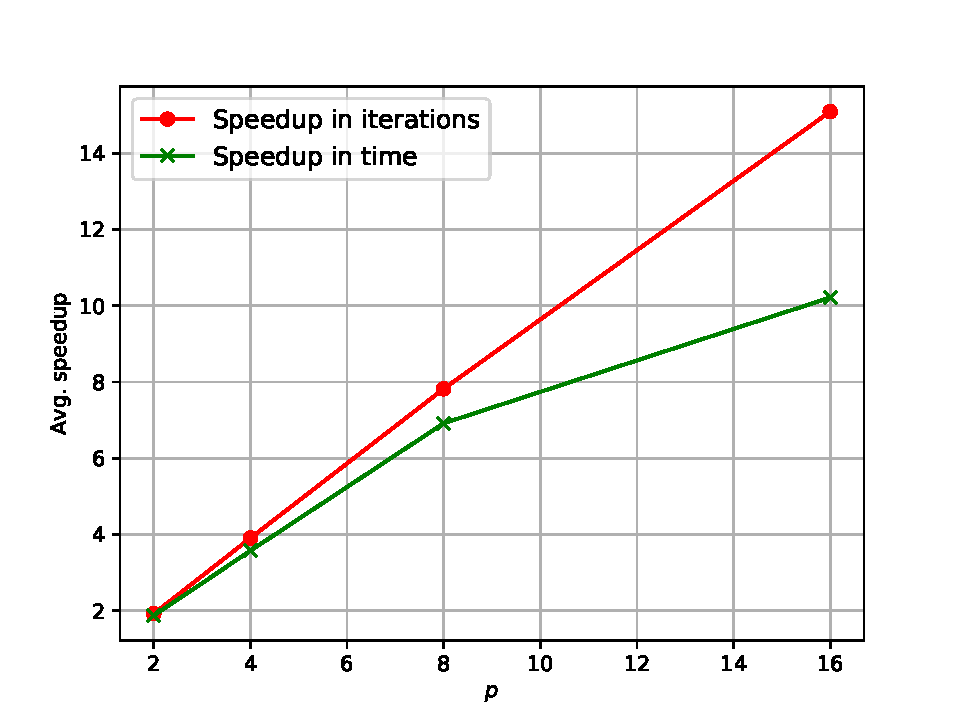
\includegraphics[width=.5\textwidth]{./img/speedup.pdf}}}
      \subfloat{{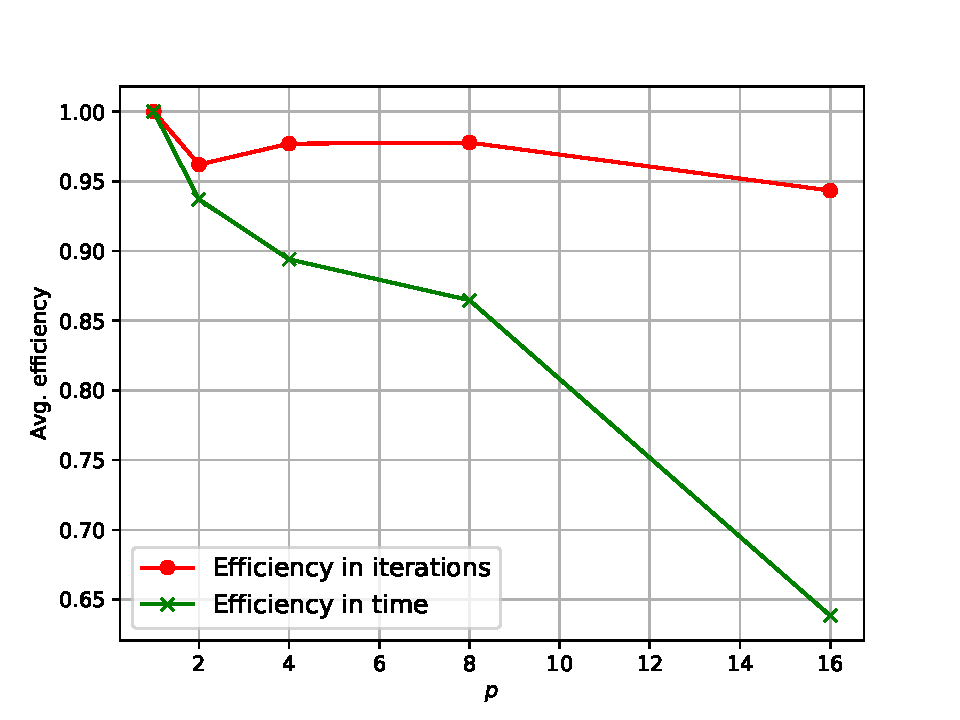
\includegraphics[width=.5\textwidth]{./img/efficiency.pdf} }}
  \end{figure}
\end{frame}

\begin{frame}
  \frametitle{Conclusion and future work}
    Already done:
    \begin{itemize}
      \item local refinement technique was introduced to the multi-objective method scheme;
      \item parallelism by characteristics was applied to the multi-objective method, efficiency metrics were collected.
    \end{itemize}
    Future work:
    \begin{itemize}
      \item compute quality metrics for the obtained solutions of the test problems;
      \item compare the method with other approaches;
      \item expand method to constrained problems;
      \item use MPI for distributed computation of objectives.
    \end{itemize}
\end{frame}

\begin{frame}{{}}
  \frametitle{ }
  \begin{center}
    \Large{Q\&A}

\vspace{1cm}

    sovrasov.vlad@gmail.com

    https://github.com/sovrasov
  \end{center}
\end{frame}

\end{document}
